\section{Definition of Process and Policy\label{sec:definition-of-process}}


Bureaucratic organizations manage shared resources (tangible or expertise). 
A subjective decision about a resource that is administered by bureaucrats is formalized as a \gls{policy}.
The policy of an organization constrains what action is required, allowed, or not allowed with respect to the shared resource being managed by the organization.

% definition
To determine which policies apply in a given circumstance, a sequence of tasks (referred to as a \gls{process}) are defined. 
% Also known as a procedure. 
In a confusingly circular dependence, tasks may invoke policy enforcement by bureaucrats. 

Processes inform the decision-making of bureaucrats and result in access to or denial of shared resources. 
A process has inputs and outputs. 
A process can be decomposed into other processes. 
Processes operate on both information and tangible objects. 
Processes require \href{https://en.wikipedia.org/wiki/Work_(physics)}{work}
\index{Wikipedia!\href{https://en.wikipedia.org/wiki/Work_(physics)}{work}}
and time. 
Processes are carried out by people or machines.

Processes are important for organizations because they create a defensible story for the bureaucrats involved. Processes are not correlated with fair distribution of the shared resource managed by the bureaucracy. Management of shared resources require policies, and implementing policies require processes. The processes are one step removed from the management of the shared resources. 


The alternative to process is an \hyperref[sec:exceptions-to-process]{exception}\iftoggle{haspagenumbers}{ -- see page~\pageref{sec:exceptions-to-process} for more details.}{.}
Creating and maintaining processes is burdensome, as is dealing with exceptions. This is the \hyperref[table:dilemma-personal-policy-consistency-across-cases]{Dilemma of Consistent Policies}\iftoggle{haspagenumbers}{; see page~\pageref{table:dilemma-personal-policy-consistency-across-cases}.}{.}

\ \\

% https://graphthinking.blogspot.com/2019/04/dealing-with-rules.html
In your role as bureaucrat or subject you have options for responding to policies and processes. You can:
\begin{itemize}
    \item Accept them. The default for most bureaucrats in an  organization.
    \item Intentionally break them maliciously (to cause harm). Typically limited to a small number of participants. These defectors have various motives -- frustration, moral opposition, personal revenge, etc.
    \item Intentionally break them for disruptive innovation. 
    From the view of other bureaucrats, your intent of innovation may be indistinguishable from malice. 
    \item Be ignorant of them. This may initially be easier for you (there's less to think about) but causes friction for everyone else and results in you being less effective. 
    \item Work in an environment where the rules have not yet been set. Then you are either limited in scale and complexity, or you will need to form new policies and processes as the organization grows.
\end{itemize}

\ \\

% process and roles
Processes are typically divided into separate tasks. With sufficient scale and complexity, each task becomes associated with distinct roles. The distinction of roles originates in skill specialization, separation of responsibilities, and enabling narrow authority. 

When there is insufficient staffing then individual bureaucrats have multiple roles. This can lead to a conflict of interest among the roles held by one person and is experienced by the bureaucrat as a \href{https://en.wikipedia.org/wiki/Cognitive_dissonance}{cognitive dissonance}. 
\index{Wikipedia!\href{https://en.wikipedia.org/wiki/Cognitive_dissonance}{cognitive dissonance}}
For example, when one person has both the responsibility to implement a plan and review the completed implementation, the oversight is ineffective.\footnote{For a formal mechanism of documenting roles, see the 
\href{https://en.wikipedia.org/wiki/Responsibility_assignment_matrix}{Responsibility Assignment Matrix}.
\index{Wikipedia!\href{https://en.wikipedia.org/wiki/Responsibility_assignment_matrix}{Responsibility Assignment Matrix}}
}

\ \\

% how does understanding process help me?
The above observations are theoretical and generic, but there's already practical relevance to your actions as a bureaucrat.
\begin{itemize}
    \item Understanding concepts like process and policy helps you know when to work within versus work around, when to accept versus change, when to ignore, how to leverage, and how to design.
    \item In your role as a bureaucrat you administer a process. When you do that, check that the person you are inflicting the process on can explain the steps back to you. If they cannot, their confusion will likely create more work for the bureaucrats involved. 
\marginpar{$>>$ Actionable Advice}
\index{actionable advice}
    \item As the subject of a process, check that your understanding of the process is consistent with the bureaucrat's intent. Summarize the next steps and applicable deadlines so they can confirm. 
\end{itemize}

\ \\

% dangers of process
The simplifications necessary for making policies and the neglect of specific circumstances results in \gls{process friction}. Process friction manifest in waste of resources (tangible or expertise), temporal inefficiency, emotional frustration, and social distrust of institutions.


%Two distinguishing features in the context of bureaucracy are authorization and justification.  

\subsection*{Types of Process}
% https://graphthinking.blogspot.com/2016/07/three-process-types-in-large-complex.html
The generic definition of \gls{process} used above obscures distinct subcategories. In practice, there are three types of processes: heroic, bureaucratic, and social.

\index{process type!heroic}
A \underline{heroic process} is exemplified by a single person or a small number of people doing the work associated with a specific task. The person may be acting in multiple roles and typically relies on expertise from multiple domains. This approach is not sustainable as there's significant dependence on the hero(s). The heroic process is a common pattern because it minimizes the work of other bureaucrats and is more efficient because there's less hand-off between bureaucrats. The heroic process may cause demoralization of the hero (because other bureaucrats are not able to reward the hard work) and result in burn-out. 

% process design trade-offs
Processes with fewer people and fewer steps can be quicker and use fewer resources, but they are more fragile and likely to be particular to the administering bureaucrat. Having more people involved helps with edge cases but slows down the process.  Hero culture is rarely an intentional design; it is based on personalities and cost to the organization. Enabling redundancy in the form of a buddy system (\href{https://en.wikipedia.org/wiki/Pair_programming}{pair programming} 
\index{Wikipedia!\href{https://en.wikipedia.org/wiki/Pair_programming}{pair programming}}
for software, \href{https://en.wikipedia.org/wiki/Standard_RAID_levels#RAID_1}{RAID 1} 
\index{Wikipedia!\href{https://en.wikipedia.org/wiki/Standard_RAID_levels}{Standard RAID levels}}
for data storage) costs more in the short term. 

The arguments against hero culture center on the long-term benefits of resilience and scalability. Those motivations lead to the next type of process.

\index{process type!bureaucratic}
A \underline{bureaucratic process} is a sequence of steps with each step administered by a different bureaucrat. The steps of the process may not be communicated to process participants, which often causes frustration when the subject of bureaucracy has to discover each step sequentially. The number of steps in the bureaucratic process may seem onerous to subjects going through the process because of the multiple interactions with different bureaucrats (compared to the heroic process). The process often takes longer than desired due to loss of information and context in the hand-off among bureaucrats. The participant has to re-explain the same background to each bureaucrat.

In contrast to heroic processes and social processes, bureaucratic processes are associated with forms (paper or electronic). 
Forms are meant to enable hand-off among bureaucrats, ensure consistent application of policy, and to catch people who shouldn't get the resource (both in cases of accidental request and malicious request). For malicious requests, a more burdensome process merely filters the low-cost grifters. 

\index{process type!social}
A \underline{social process} is undocumented and relies on relationships instead of hierarchy. There is a strong sensitivity to prior experiences of the bureaucrats and on the skills of the people involved. There is no single person that represents or manages the social network, so the entry point is through relationships with bureaucrats who have existing connections.

Once distinctions between heroic, bureaucrats, and social processes are recognized, tactics can be used to address the challenges associated with each type of process.

If you are blocked by the hero of a heroic process, you can try waiting until the hero leaves. Given burn-out and turnover, sometimes this is only a few years. Alternatively, you can try creating a positive relationship with the hero.  If you're the hero and don't want to be, look for ways to transition to bureaucratic or social processes. 


For the social process, participants are swayed by reputation more than title. In an ideal bureaucratic process your reputation wouldn't matter. That assumption turns out to not be valid. Building and maintaining relationships matters for all three types of process.
%Prestige and reputation matter. 
\begin{itemize}
    \item Learn the interests and dislikes of your coworkers involved in processes you care about.
    \item Doing favors for process participants acts as professional lubricant. However, explicit quid pro quo is likely to fail due to inadequate trust. 
    \item Bring cookies and donuts and brownies to foster relationships and good will. 
\marginpar{$>>$ Actionable Advice}
\index{actionable advice}
Instead of bringing food when a favor is needed, bring food on a recurring basis before the favor is needed. Again, trust is built of over time. 
\end{itemize}

Social processes can work well for small tasks that are infrequent.
Social processes can be effective in anomalous situations.
Bureaucratic processes are useful under typical conditions.

When you are forced to use a bureaucratic process for a complex objective and you have not previously used the process, avoid using the critical case for learning. Instead of starting with the most important or hardest problem, send a test case through the process. This enumerates the sequence of steps, provides a measure of the time needed to get through the process, and identifies key personnel. 

Thinking of bureaucratic processes in opposition to social relationships is a false dichotomy. Bureaucratic processes are formalized versions of interactions intended to displace the need for social relationships among bureaucrats.
% https://graphthinking.blogspot.com/2021/04/laffer-curve-and-minimum-viable.html
When no process exists, only people with relationships succeed. Processes enable novices to an organization to contribute value and gain experience. 



Processes (whether heroic, bureaucratic, or social) are not consistent because relationships vary -- both among the bureaucrats administering the process and the person going through the process.






\begin{figure}
    \centering
    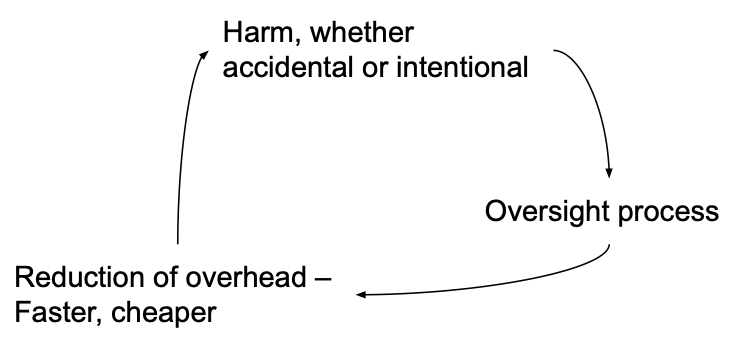
\includegraphics{images/process_loop_harm-oversight-improvement}
    \caption{The harm-oversight-improvement loop that motivates policies and processes.}
    \label{fig:harm-oversight-improvement}
\end{figure}







% Process discovery: Detect whether a process exists. 

% https://graphthinking.blogspot.com/2015/07/notes-on-bureaucracy-and-social-network.html
%Do participants know about existing processes?

%Processes can be undocumented. Then oral folklore is the mechanism. 

